\documentclass[conference]{IEEEtran}
\IEEEoverridecommandlockouts
% The preceding line is only needed to identify funding in the first footnote. If that is unneeded, please comment it out.
\usepackage{cite}
\usepackage{amsmath,amssymb,amsfonts}
\usepackage{graphicx}
\usepackage{textcomp}
\usepackage{xcolor}
\usepackage {enumitem}
\def\BibTeX{{\rm B\kern-.05em{\sc i\kern-.025em b}\kern-.08em
    T\kern-.1667em\lower.7ex\hbox{E}\kern-.125emX}}
\title{
\vspace{1cm}
{\includegraphics[width=0.15\textwidth]{/storage/emulated/0/Screenshot_2024_1018_113636.jpg} \\ 7447 BCD-Seven Segment Display decoder} }
\author{Shaik Mohisena Tabassum \\ Roll No: FWC22279 \\ shaikmohisena123@gmail.com}
 \begin{document}
\maketitle
 \section {ABSTRACT}
 The document shows how to use the 7447 BCD-Seven Segment Display decoder to learn boolean logic.
\section{COMPONENTS}
The required components list is given in Table: I. The pin diagram of the seven segment display is shown in Fig.1. \\
The pin diagram of IC 7447 is shown in Fig.2 
 \begin{table} [htbp]
\centering
\begin{tabular}{| c | c | c |} \hline
\textbf{Components} & \textbf{Value} & \textbf{Quantity} \\\hline
Seven Segment Display & & 1 \\ \hline
IC & 7447 & 1 \\ \hline 
Arduino & UNO & 1 \\ \hline
Jumper Wires &  & 10 \\ \hline
Breadboard & & 1 \\ 
\hline
\end{tabular}
\vspace{0.1cm}
\caption{\label{tab:widgets}}
\end{table}
\vspace {0.1cm}
\begin{figure}[h]                                
\centering                                       
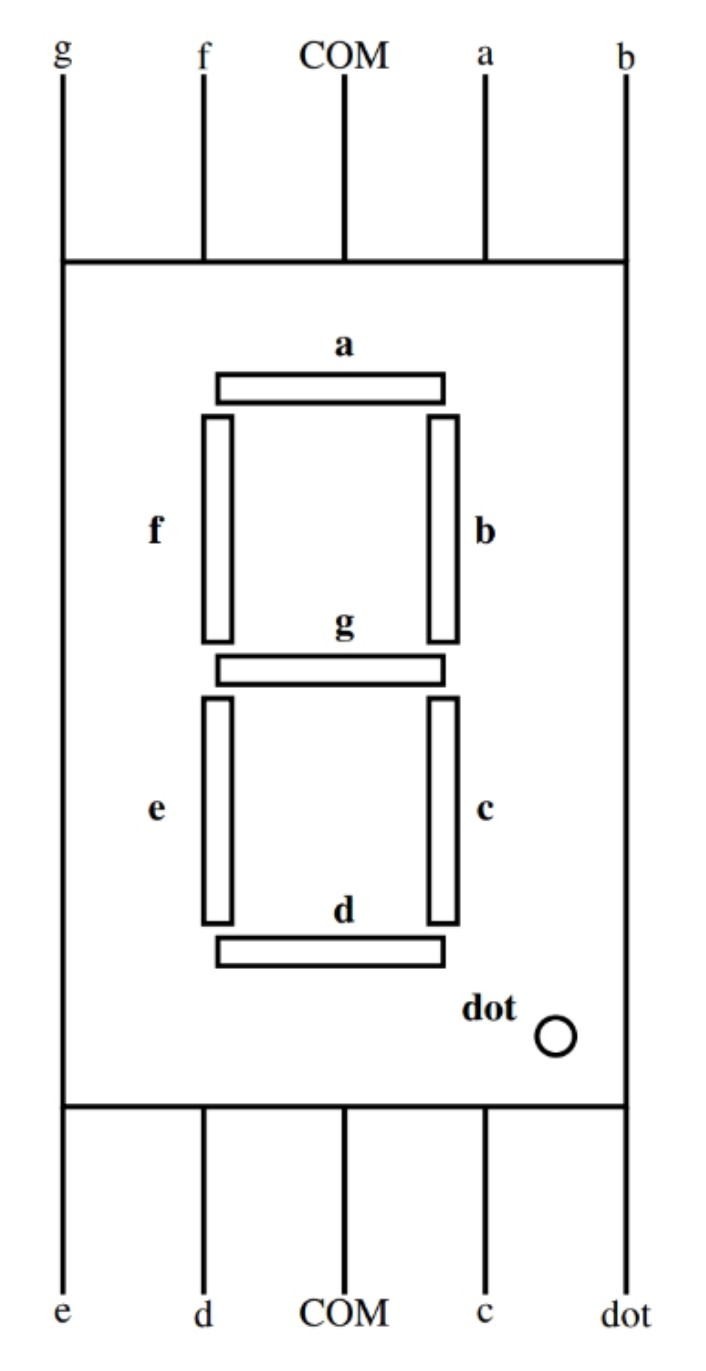
\includegraphics[width=0.15\textwidth]{Screenshot_2024_1021_104340.jpg}                            
\caption{\label{fig:Gates}}                    
\end{figure}

\begin{figure}[h]
\centering
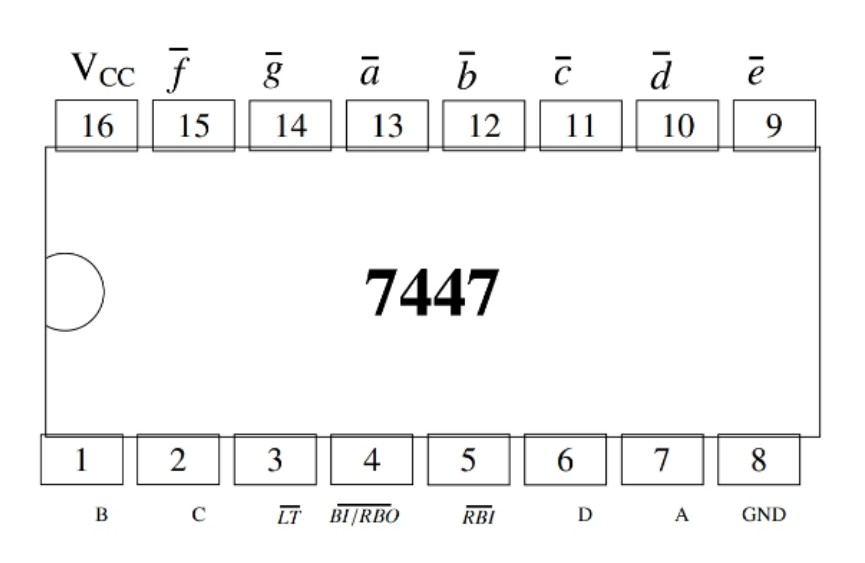
\includegraphics[width=0.35\textwidth]{/storage/emulated/0/internship/Screenshot_2024_1021_112333.jpg}
\caption{\label{fig:Gates}}
\end{figure}

\section{PROCEDURE}
\begin {enumerate}
\item Make the connections between 7447 and Seven segment display as per the Table: II.
\begin{table}                       
\centering                          
\begin{tabular}{| c | c | c | c | c | c | c | c |} \hline                                
	\textbf{7447} & $\overline{a}$ & $\overline{b}$ & $ \overline{c}$ & $\overline{d}$ & $\overline{e}$ & $\overline{f}$  & $\overline{g}$ \\\hline 
\textbf{Display} & a & b & c & d & e & f & g \\ \hline                           
\end{tabular}             
\vspace{0.1cm}                                 
\caption{\label{tab:widgets}}                     
\end{table}
\item Make the connections between Arduino and 7447 as per the Table: III.

\begin{table} 
\centering
\begin{tabular}{| c | c | c | c | c |} \hline
\textbf{7447} & $D$ & $C$ & $B$ & $A$ \\\hline
\textbf{Arduino} & $5$ & $4$ & $3$ & $2$ \\ \hline 
\end{tabular}
\vspace{0.1cm}
\caption{\label{tab:widgets}}
\end{table}
\item The truth table for the increment decoder is shown in Table IV.

\begin{table} [htbp]
\centering
\begin{tabular}{| c | c | c | c | c | c | c |c |} \hline
$Z$ & $Y$ & $X$ & $W$ & $D$ & $C$ & $B$ & $A$ \\\hline
$0$ & $0$ & $0$ & $0$ & $0$ & $0$ & $0$ & $1$ \\ \hline 
$0$ & $0$ & $0$ & $1$ & $0$ & $0$ & $1$ & $0$ \\ \hline
$0$ & $0$ & $1$ & $0$ & $0$ & $0$ & $1$ & $1$ \\ \hline
$0$ & $0$ & $1$ & $1$ & $0$ & $1$ & $0$ & $0$ \\ \hline
$0$ & $1$ & $0$ & $0$ & $0$ & $1$ & $0$ & $1$ \\ \hline
$0$ & $1$ & $0$ & $1$ & $0$ & $1$ & $1$ & $0$ \\ \hline
$0$ & $1$ & $1$ & $0$ & $0$ & $1$ & $1$ & $1$ \\ \hline
$0$ & $1$ & $1$ & $1$ & $1$ & $0$ & $0$ & $0$ \\ \hline
$1$ & $0$ & $0$ & $0$ & $1$ & $0$ & $0$ & $1$ \\ \hline
$1$ & $0$ & $0$ & $1$ & $0$ & $0$ & $0$ & $0$ \\ \hline
\end{tabular}
\vspace{0.1cm}
\caption{\label{tab:widgets}}
\end{table}

\item Run the code. And observe the output in the display as in Fig.3.

\end {enumerate}                     
\section{RESULTS}
Download the code given in the link below and execute them to see the output as shown in Fig.3 by observing in seven segment display. 
\\ https://github.com/Tabassum4930/FWC-1/blob/main/Ide/7447/code.cpp
\begin{figure}[h] 
	\centering 
	\includegraphics[width=0.35\textwidth]{/storage/emulated/0/internship/7447.jpg}
	\caption{\label{fig:Gates}}    
\end{figure}
\section{CONCLUSION}
Therefore, it is an essential component in the experimentation of digital circuits.
\end{document}
